\documentclass[a4paper, 11pt]{article}
\usepackage[utf8]{inputenc}
\usepackage[ngerman]{babel}
\usepackage{graphicx}
\usepackage{color}
\usepackage{tikz}
\usepackage{pgfplots}
\usepackage{amssymb}
\pagestyle{headings}
\usepackage{eurosym}


\begin{document}

\title{Exakte Lösung von TSP-Problemen}
\author{Axel Christ\\
  DHBW Karlsruhe,\\
  TINF12B2,\\
  Seminar Theoretische Informatik}
\date{\today}
\maketitle
\newpage

\tableofcontents
\newpage

Das Travelling-Salesman Problem

\section{Einleitung}

\subsection{Geschichte}

Das Travelling-Salesman Problem ist ein Problem, das schon seit der Antike
besteht und die Menschen (und heute auch Maschinen) zum Nachdenken bringt:
Ein Bote/Handlungsreisender muss mehrere Städte besuchen und möchte den
kürzesten Weg finden, mit dem er jede Stadt exakt einmal in einer geschlossenen
Tour besuchen kann. \\

Wann das Problem ein erstes mal wissenschaftlich untersucht wurde ist unklar,
jedoch gab es im Jahre 1832 ein Handbuch für Handlungsreisende, das das Problem
zwar erwähnt aber nicht weiter behandelt.\\

Erstmals als Optimierungsproblem wurde das TSP im Jahre 1930 vom österreichischen
Mathematiker Karl Menger unter dem Titel \textit{Botenproblem}. Schon im
Vorhinein dieser Erwähnung gab es das \textit{Icosian Game} von William Rowan
Hamilton, der in einem Graphen Touren zwischen 20 Knoten finden wollte.\\

\subsection{Einsatzbereiche und Klassifikationen}

Heute hat das Travelling-Salesman Problem noch weitere, wichtige Einsatzbereiche
dazubekommen: So ergeben sich ähnliche Probleme bei der Genom-Sequenzierung, bei
der optimalen Plazierung von Bauteilen bei der Konzeption von Mikrochips, bei
der Tourenplanung von Logistikrobotern in großen Versandzentren (siehe Amazon)
oder bei der Tourplanung von Satelliten im Weltall um Sternenbilder zu erstellen.\\

Das Travelling-Salesman Problem selbst kann auch in mehreren Varianten (z.B.
bei einigen der vorher genannten Einsatzbereiche) auftreten. Eine mögliche
Variation ist das \textit{multiple TSP}, bei dem die Städte zusätzlich auf
mehrere Handlungsreisende aufgeteilt wird, wobei die Touren aller Reisenden
in der gleichen Stadt starten und enden müssen. Das multiple TSP kann noch
über das zusätzliche Kriterium, dass jeder Handlungsreisende mindestens zwei
Städte besuchen muss, zum schwierigeren \textit{multiple TSP with nonlazy
Salesmen} verschärft werden. Eine andere erwähnenswerte Variante ist das
\textit{Vehicle Routing Problem}, bei dem zusätzlich zu dem multiple TSP
Transportrestriktionen, wie z.B. Ladekapazitäten eines LKWs berücksichtigt werden
müssen. Weitere Variationen existieren, auf diese wird hier jedoch nicht näher
eingegangen.

\subsection{Schwierigkeiten}

Das Problem ist somit wichtig für viele Anwendungen, jedoch ist es bis heute
schwer, das Travelling-Salesman Problem exakt zu lösen: 1972 wurde die
\textit{NP-Vollständigkeit} des Hamiltonkreisproblems \footnote{
  Das Hamiltonkreisproblem beschreibt die Schwierigkeit einen
  geschlossenen Pfad in einem Graphen zu bestimmen, der jeden Knoten genau
  einmal enthält.
} festgestellt, aus dieser Feststellung ließ sich die NP-Vollständigkeit
des TSPs einfach herleiten. \\

In der folgenden Zeit bis heute wurden viele Anstrengungen unternommen, um das
TSP zu lösen oder zumindest näherungsweise zu bestimmen. Einige namhafte Algorithmen
zur näherungsweisen (auch möglicherweise optimalen) Lösung hierunter sind der
\textit{Kernighan-Lin-Algorithmus} oder auch \textit{Genetische Algorithmen}. Im
Folgenden soll aber genauer auf die Optimalen Verfahren wie auch teilweise auf deren
mathematische Grundlagen eingegangen werden.

\section{Analyse}

\subsection{Mathematische Betrachtung}

Im vorangehenden wurde oft der Begriff Städte für die Punkte verwendet, die
ein Handlungsreisender besuchen muss. Für die allgemeinere Definition wird
nun der Begriff \textit{Knoten} verwendet. \\

Ein TSP-Problem hat $N$ Knoten aus der Knotenmenge $V$. Zwischen allen Knoten
gibt es eine Verbindung, im Folgenden Kante genannt. Falls im ursprünglichen
Modell keine solche Kante existiert, so wird eine mit großer Länge eingefügt.
Zu jeder Kante zwischen einem Knoten $i$ und einem Knoten $j$ gibt es eine
Länge $c_{i,j} \geq 0$. \\

Um eine Tour zu beschreiben wird für jede Kante eine boolesche Variable $x_{i,j}$
eingeführt, wobei $i$ und $j$ jeweils unterschiedliche Knoten sind. Falls eine
Kante in einer Tour enthalten ist, so ist diese boolesche Variable $x = 1$,
ansonsten ist sie $0$. \\

Diese Bedingungen alleine genügen jedoch nicht: Falls man es nicht definieren
würde, wären somit Touren möglich, die durch einige Knotenpunkte mehrfach laufen
würden (siehe \ref{fig:multiple_connections_per_node}). Um solche Touren zu
vermeiden definiert man folgendes:

$$\sum_{j \in V \backslash i}x_{i,j} = 2$$

Die Summe aller Kanten, die in einen Knoten gehen, muss stets zwei sein (eine
eingehende und eine ausgehende Kante). \\

\begin{figure}[p]
    \centering
    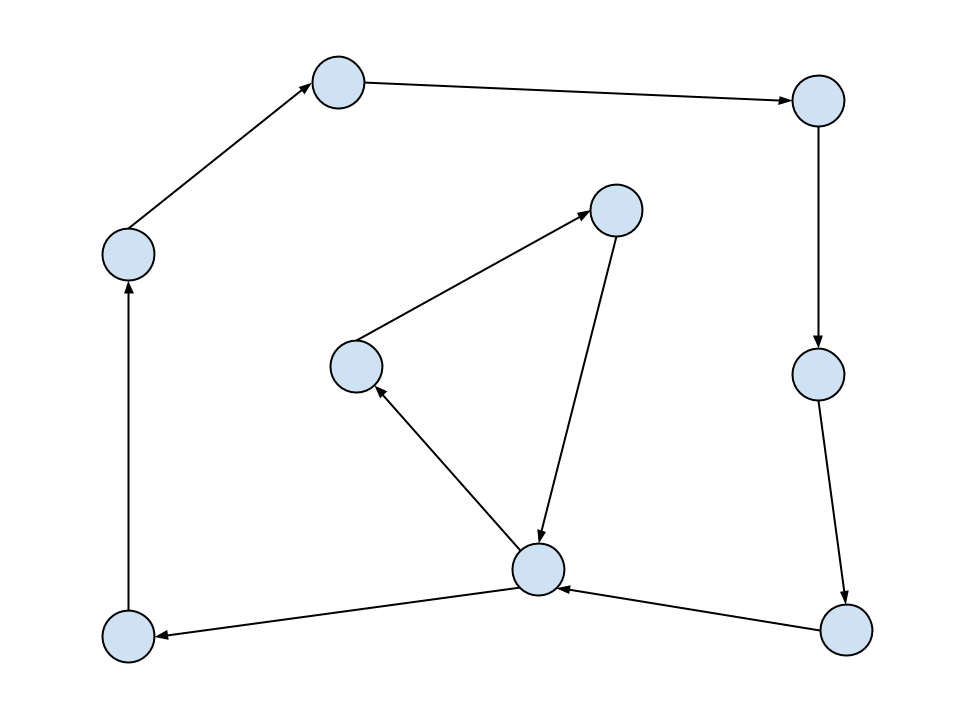
\includegraphics[width=0.8\textwidth]{invalid_tour.png}
    \caption{Drei Kanten zu einem Knoten}
    \label{fig:multiple_connections_per_node}
\end{figure}

Dennoch muss noch eine Bediungung definiert werden, damit eine Tour valide ist:
Momentan wäre eine Tour wie in \ref{fig:short_cycles} möglich, die sogenannte
\textit{Kurzkreiszyklen} enthält. Kurzkreiszyklen verletzen die Bedingung der
ein- und ausgehenden Kanten pro Knoten zwar nicht, jedoch entsteht so keine
zusammenhängende Tour. Um solche Touren zu verhindern definiert man deshalb
folgende Nebenbedingung:

$$\sum_{i \in S, j \notin S}x_{i,j} \geq 2$$

Hierbei werden zwei Mengen definiert: $S$ und $S^C$ (in der Formel mit
$j \notin S$). Eine Knotenmenge $V$ kann in $2^N$ verschiedene Mengen zerlegt
werden, weshalb man mit dieser Bedingung $2^N$ Nebenbedingungen hinzufügen
würde. Mathematisch gesehen ist diese Bedingung zwar zwingend notwendig, 
einige Programme zur Lösung eines TSPs fügen diese Bedingungen aber erst
dynamisch zur Laufzeit Schritt für Schritt hinzu. \\

Hat man nun eine valide Tour, so ist die Aufgabe, die Gesamtlänge der Tour
zu minimieren:

$$min\sum_{i \in V} \sum_{j \in V \backslash i} c_{i,j}x_{i,j}$$

\begin{figure}[p]
    \centering
    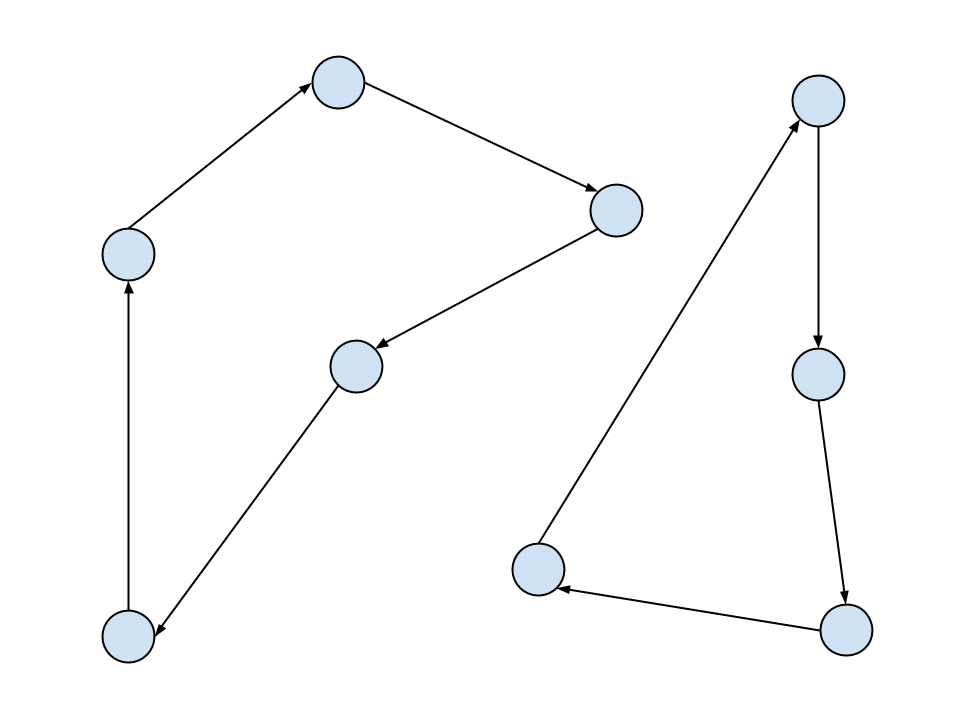
\includegraphics[width=0.8\textwidth]{kurzkreiszyklen.png}
    \caption{Kurzkreiszyklen innerhalb einer Tour}
    \label{fig:short_cycles}
\end{figure}

\subsection{Klassifikationen}

Wie schon zuvor gesehen, kann ein TSP in verschiedenen Variationen auftreten.
Es existieren deshalb einige Klassifikationen für TSPs:

\begin{itemize}
  \item Symmetrische TSPs sind TSPs bei denen der Hin- und der Rückweg stets
  gleich lang ist. Mathematisch wird dies beschrieben durch
  $c_{i,j} = c_{j,i}$. Ein TSP, das symmetrisch ist, ist beispielsweise das
  \textit{Euklidische TSP}, bei dem Knoten Punkte im zweidimensionalen Raum
  sind.

  \item Das ``Gegenstück'' zu symmetrischen TSPs sind asymmetrische TSPs.
  Bei diesen TSPs muss die Bedingung, dass Hin- und Rückweg gleich lange
  sind, nicht immer erfüllt sein. Ein asymmetrisches TSP ist z.B. im Alltag
  gegeben, wenn man beim Hinweg über Einbahnstraßen relativ direkt von A
  nach B kommt, aber man beim Rückweg diese Einbahnstraßen nicht nutzen kann.

  \item Metrische TSPs erfüllen die \textit{Dreiecksungleichung}. Die
  Dreiecksungleichung lautet $c_{i,j} \leq c_{i,k} + c{k, }$ und beschreibt,
  dass eine Strecke von einem Punkt $i$ zum Punkt $j$ immer kürzer sein
  muss als die Strecke über einen dritten Punkt $k$. Ein nicht-metrisches
  TSP ist gegeben, wenn beispielsweise Umrüstzeiten berücksichtigt werden
  müssen.
\end{itemize}

\subsection{Komplexität}

Die Anzahl der Touren bei einem asymmetrischen TSP sind $(N - 1)!$ (
Entscheidungsbaum pro Kante). Bei einem symmetrischen TSP gibt es
$\frac{N - 1}{2}$ Touren (da der Hin- und Rückweg zwischen zwei Kanten
derselbe ist halbiert sich die Anzahl der möglichen Touren).\\

Falls man sich einmal nicht in einem euklidischen TSP befindet muss man
auch die Kantenlängen errechnen. Würde man dies für ein Problem mit
$N = 1000$ (1000 Städte) tun, so hätte man erst einmal 1.000.000 mögliche
Verbindungen. Diese Für jede dieser Verbindungen müsste man, z.B. bei einem
Straßennetz, einen Dijkstra-Durchlauf starten. Ein Dikjstra-Durchlauf benötigt
bei beispielhaften Bedingungen ca. 10s, daraus resultiert eine Laufzeit von $\approx$
116 Tagen. In der Praxis verwendet man deshalb häufig die Luftlinie zwischen
zwei Städten multipliziert mit $1.3$ als Approximation (für die meisten
Umgebungen hinreichend genau).

\section{Exakte Lösungen}

\subsection{Permutation}

Das TSP kann gelöst werden, indem man durch alle möglichen Touren permutiert.
Für kleine $N$ ist dies noch möglich, jedoch die Anzahl an Touren wächst
drastisch mit größeren Knotenanzahlen (siehe \ref{fig:faculty_graph}). Ein
effizienteres Verfahren muss also bestimmt werden.

\begin{figure}
  \centering
  \begin{tikzpicture}[scale=0.6]
    \begin{axis}[
        symbolic x coords={3, 4, 5, 6, 7, 8},
        xtick=data
      ]
        \addplot[ybar,fill=blue] coordinates {
            (3, 1)
            (4, 3)
            (5, 12)
            (6, 60)
            (7, 360)
            (8, 2520)
        };
    \end{axis}
  \end{tikzpicture}
  \label{fig:faculty_graph}
  \caption{Anzahl Touren in Abhängigkeit $n$ bei symmetrischem TSP}
\end{figure}

\subsection{Lineare Programmierung}

Ein Verfahren, das bei erster Betrachtung nicht als ein Verfahren zur Lösung
des TSPs anmutet, ist die Lineare Programmierung. Bei der Linearen Programmierung
werden Probleme mit einer Zielfunktion und mehreren Nebenbedingungen,
sogenannten \textit{Constraints} gelöst.

\subsubsection{Mathematische Beschreibung}
Bei einem linearen Programm ist eine Matrix $A \in \mathbb{R}^{m,n}$ sowie
zwei Vektoren $b \in \mathbb{R}^m$ und $c \in \mathbb{R}^n$ gegeben. Der
Vektor $b$ formuliert die Constraintwerte, $c$ die Zielfunktion und $A$ die
einzelnen Constraintgleichungen. Ziel ist es, einen
zulässigen Vektor $x$ zu finden, der das Standardskalarprodukt
$c^Tx = c_1x_1 + \ldots + c_nx_n$ maximiert. Falls man minimieren statts
maximieren will, so multipliziert man $c$ mit $-1$. 

\paragraph{Beispiel}
Ein Beispiel zu einem Problem der linearen Programmierung ist die Produktionsplanung
einer Möbelfirma:

Diese Möbelfirma stellt zwei unterschiedliche Sofas her: Ein normales und ein
Sondermodell.

Pro normalem Modell verdient die Firma 500\euro, ein Sondermodell bringt 300\euro.

Die Herstellung des regulären Modells benötigt zwei Stunden, die des Sondermodells
drei.

Drei Arbeiter arbeiten pro Tag jeweils 8 Stunden für die Möbelfabrik.

Der Bedarf an normalen Sofas pro tag ist maximal sechs, bei den Sondermodellen werden
täglich maximal acht benötigt.

Die Optimierungsaufgabe hierbei ist es, den Profit der Möbelfirma zu maximieren.
Um dieses Ziel zu erreichen, muss man zunächst die Zielfunktion und die Constraints
herauslesen. In diesem Falle sind die Constraints folgende:

\begin{enumerate}
  \item Arbeitszeit der Arbeiter: Jeder Arbeiter arbeitet täglich 8 Stunden,
  somit stehen insgesamt $3 \cdot 8 = 24$ Stunden für die Herstellung von
  Sofas pro tag. Da das Standardsofa $x$ jeweils zwei Stunden für die Herstellung
  benötigt und das Sondersofa $y$ jeweils drei Stunden, lässt sich daraus folgende
  Gleichung formulieren:
  $$2x + 3y \leq 24$$

  \item Nachfrage: Da vom Standardsofa maximal sechs Stück und vom Sondersofa
  maximal acht Stück benötigt werden, dürfen die Werte für $x$ und $y$ nicht
  größer als die entsprechenden Randwerte werden:
  $$x \leq 6$$
  $$y \leq 8$$

  \item Nicht-Negative Werte: Eine Randbedingung, die sich etwas schwieriger
  ablesen lässt, aber auch erforderlich ist, ist, dass die Werte für $x$ und $y$
  jeweils nicht negativ sein dürfen. Somit gilt noch:
  $$x \geq 0$$
  $$y \geq 0$$
\end{enumerate}

Zusätzlich zu den Constraintwerten muss auch die Zielfunktion bestimmt werden.
Die Zielfunktion stellt die Maximierung des Profits durch verkaufte Einheiten dar:

$$f(x) = 500x \cdot 300y$$

Grafisch würde das Problem wie in Abbildung \ref{img:graphical_problem} aussehen
(die grünen Punkte stellen ganzzahlige Lösungen dar).
\begin{figure}
  \centering
  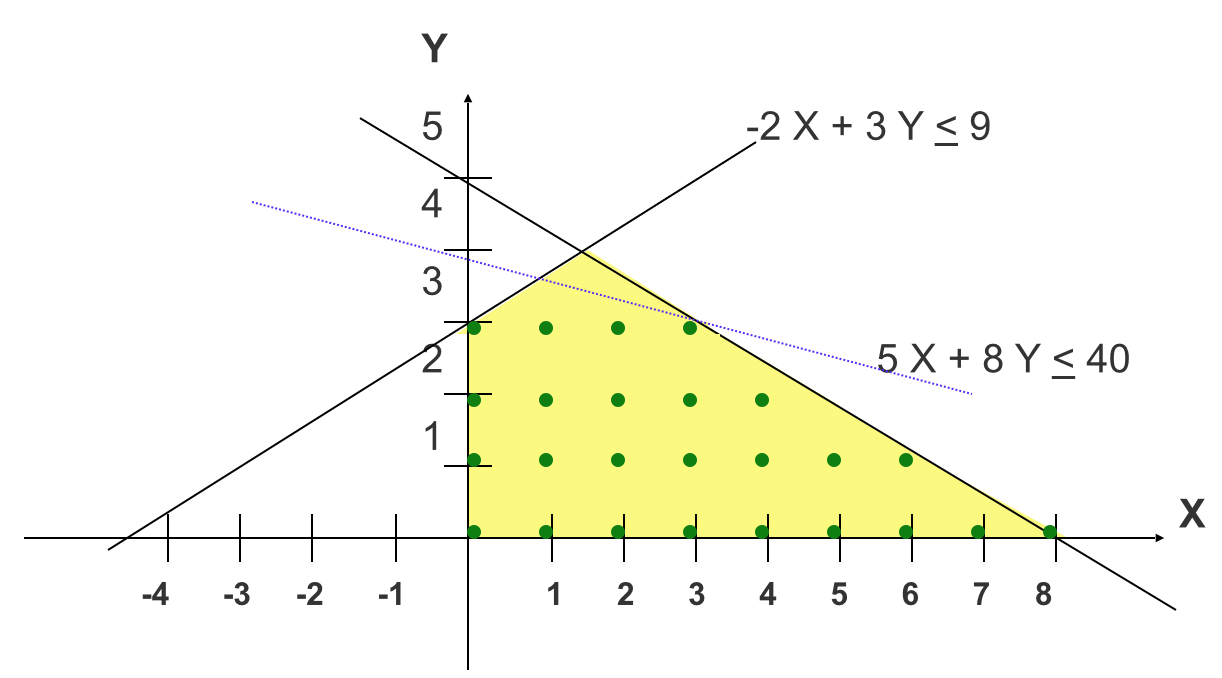
\includegraphics[width=\linewidth,height=150px,keepaspectratio]{example_graphical_representation.png}
  \caption{Problemdarstellung Produktionsplanung}
  \label{img:graphical_problem}
\end{figure}

\subsubsection{Simplex-Algorithmus}
Wie kann nun dieses Problem gelöst werden? Generell sind bei Optimierungsproblemen
die Lösungen immer an den Kanten des zulässigen Raumes. Ein Algorithmus, der dieses
Problem auch für Gleichungen mit mehr als zwei Dimensionen wie im vorher beschriebenen
Problem löst (1. Dimension: Standardsofa $x$, 2. Dimension: Sondersofa $y$) ist der
sogenannte \textit{Simplex-Algorithmus}. Stellt man sich den Lösungsraum eines
$n$-dimensionalen Problems als ein $n$-dimensionales Polyeder vor, so beginnt
der Simplex-Algorithmus mit einer Ecke (einer zulässigen Startlösung) und springt
solange von Ecke zu Ecke des Polyeders, wie keine Verbesserung mehr möglich ist.
Der Simplex-Algorithmus hat zwar eine schlechtere Laufzeit als manche andere Methoden
(wie z.B. das \textit{Innere-Punkte-Verfahren}), jedoch kann mit dem Simplex-Algorithmus
eine berechnete Lösung beim Hinzufügen einer Constraint-Bedingung verwendet werden,
was dem Simplex-Algorithmus einen erheblichen Laufzeitvorteil gibt.

\subsubsection{Branch and Bound}
Würde man nun mit dem Simplex-Algorithmus eine Lösung für das Sofaproblem berechnen,
so würde man auf eine Lösung im kontinuierlichen treffen, wie etwa $x = 1,78$ und
$y = 2,97$. Diese Lösung ist für die Praxis untauglich, da keine $1,78$ Standardsofas,
sondern nur ganze Sofas verkauft werden können. Wie kann man nun also auf ganzzahlige
Lösungen ausgehend von der Lösung im kontinuierlichen gelangen?
Ein Verfahren hierfür ist das sogenannte \textit{Branch and Bound}. Bei Branch
and Bound ist der Ausgangspunkt eine relaxierte Lösung im kontinuierlichen,
wie etwa die oben genannte Lösung mit $x = 1,78$ und $y = 2,97$.
Basierend auf dieser Lösung wird in einem Schritt in einen Bereich größer
gleich der nächsten Ganzzahl und in einen kleiner gleich der nächsten
Ganzzahl verzweigt. Für $x = 1,78$ wird somit in $x \leq 1$ und in $x \geq 2$
verzweigt (siehe \ref{img:branching}).

\begin{figure}
  \centering
  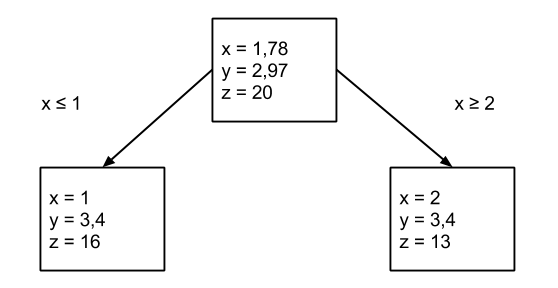
\includegraphics[width=\linewidth,height=150px,keepaspectratio]{branching.png}
  \caption{Beispiel Branching}
  \label{img:branching}
\end{figure}

Die Verzweigungsbedingung wird jeweils in die Constraintbedingungen
der weiteren Ausführungsstränge mit aufgenommen. In diesen Substrängen wird
dann wiederrum eine (möglicherweise nicht ganzzahlige) Lösung berechnet,
z.B. mit dem Simplex-Algorithmus. Alle Lösungen eines Stranges können, im Bezug
auf ihre Güte in der Zielfunktion, nicht besser als die relaxierte
Lösung $z$ der Verzweigung sein. Somit kann man hier auch wiederrum Verzweigungen
einschränken, indem man die Optimalitätsschranke mit einem bisherigen Ergebnis
vergleicht. Sollte etwa ein Strang schon ein Ergebnis mit z.B. dem Wert $13$
geliefert haben, so kann man alle Stränge verwerfen, deren Optimalitätsschranke
$\leq 13$ ist. Die Teilstränge werden somit nun immer weiter verzweigt, solange
sie nicht unter eine Optimalitätsschranke fallen (bei einer bisher gefundenen
Lösung) bis eine ganzzahlige Lösung gefunden wird.

Zusammenfassend lässt sich das Verfahren somit wie folgt beschreiben:

\begin{enumerate}
  \item Berechnen einer relaxierten Lösung mittels eines Algorithmus
  zur Lösung eines Linearen Problems, z.B. Simplex
  \item Falls Lösung $z_{neu} \leq z_{bereits gefunden}$ kannn dieser
  Strang bereits abgebrochen werden
  \item Falls Lösung nicht ganzzahlig: Weiteres Verzweigen und zurück
  zu 1., falls Lösung
  ganzzahlig: beenden dieses Stranges mit Lösung $z_{neu}$
\end{enumerate}

Eine Verzweigung kann auch zu keiner Lösung führen wenn sie außerhalb
dem erlaubten Lösungsbereich ist. In diesem Fall gibt es für einen Substrang
keine Lösung $z$.
Das Branch and Bound Verfahren führt zwar zu einer Lösung (oder auch keiner,
falls es keine Lösung gibt) aber dafür sind möglicherweise viele Verzweigungen
notwendig. Da bei jeder Verzweigung ein LP gelöst werden muss, schießt
die Laufzeit des gesamten Verfahrens in die Höhe.

\subsubsection{Schnittebenenverfahren}
Das Schnittebenenverfahren (engl. \textit{Cutting planes}) ist eine andere
Methode der Linearen Programmierung. Hierbei ist der Startpunkt des Verfahrens
ebenfalls eine relaxierte Lösung (siehe \ref{img:cutting_planes_1}),
es sollen aber nun schrittweise Schnittebenen
in Form von Nebenbedingungen hinzugefügt werden, um die letzte, nicht-ganzzahlige Lösung
abzuschneiden (siehe \ref{img:cutting_planes_2}).

\begin{figure}
  \centering
  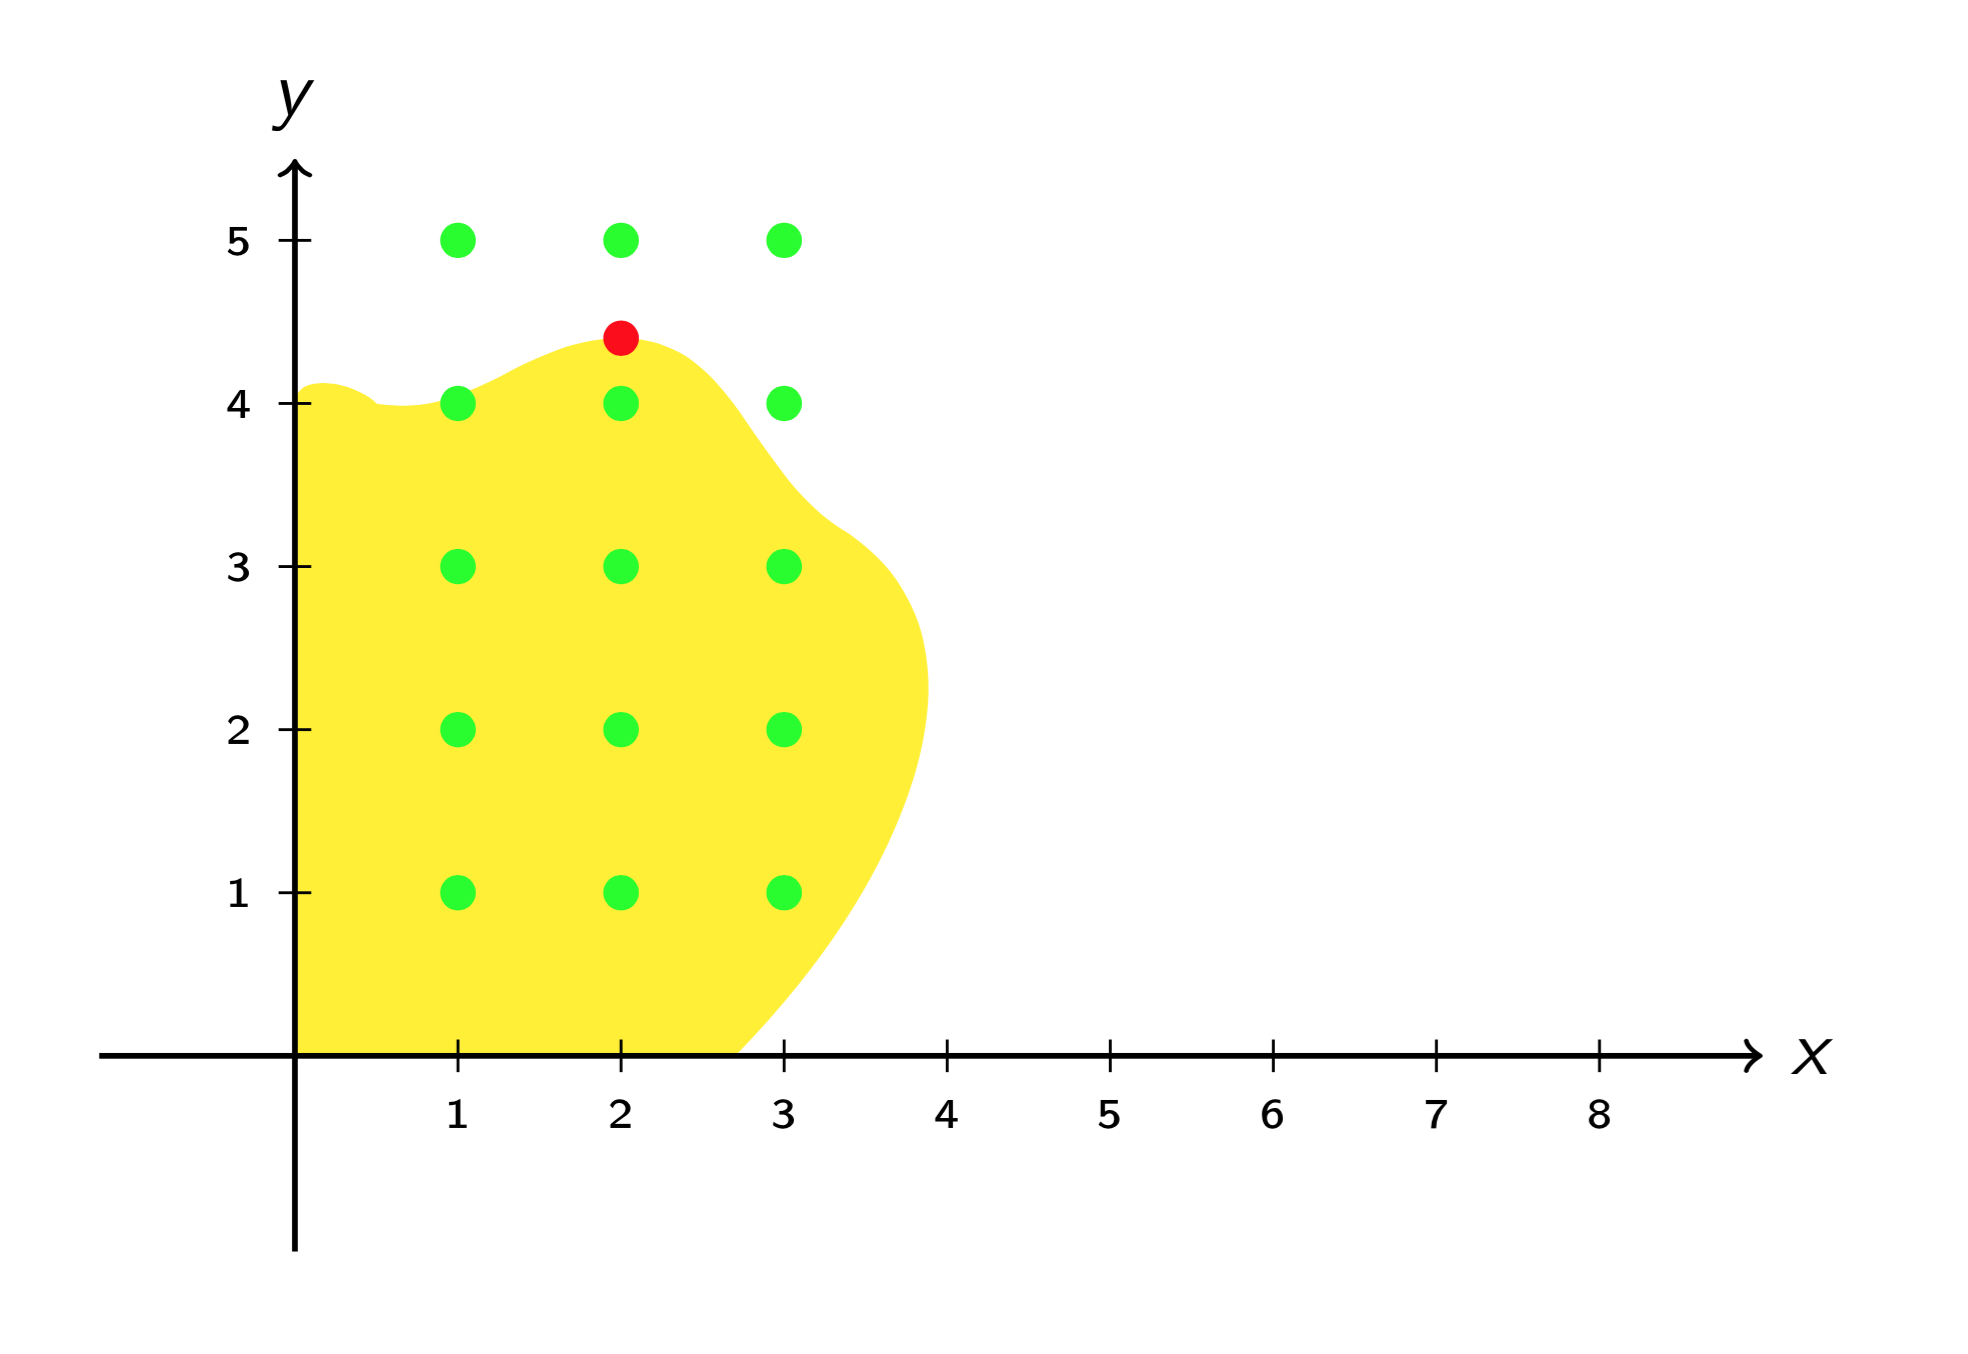
\includegraphics[width=\linewidth,height=150px,keepaspectratio]{schnittebenen_1.png}
  \caption{Ausganslösung und Lösungsraum Schnittebenenverfahren}
  \label{img:cutting_planes_1}
\end{figure}

\begin{figure}
  \centering
  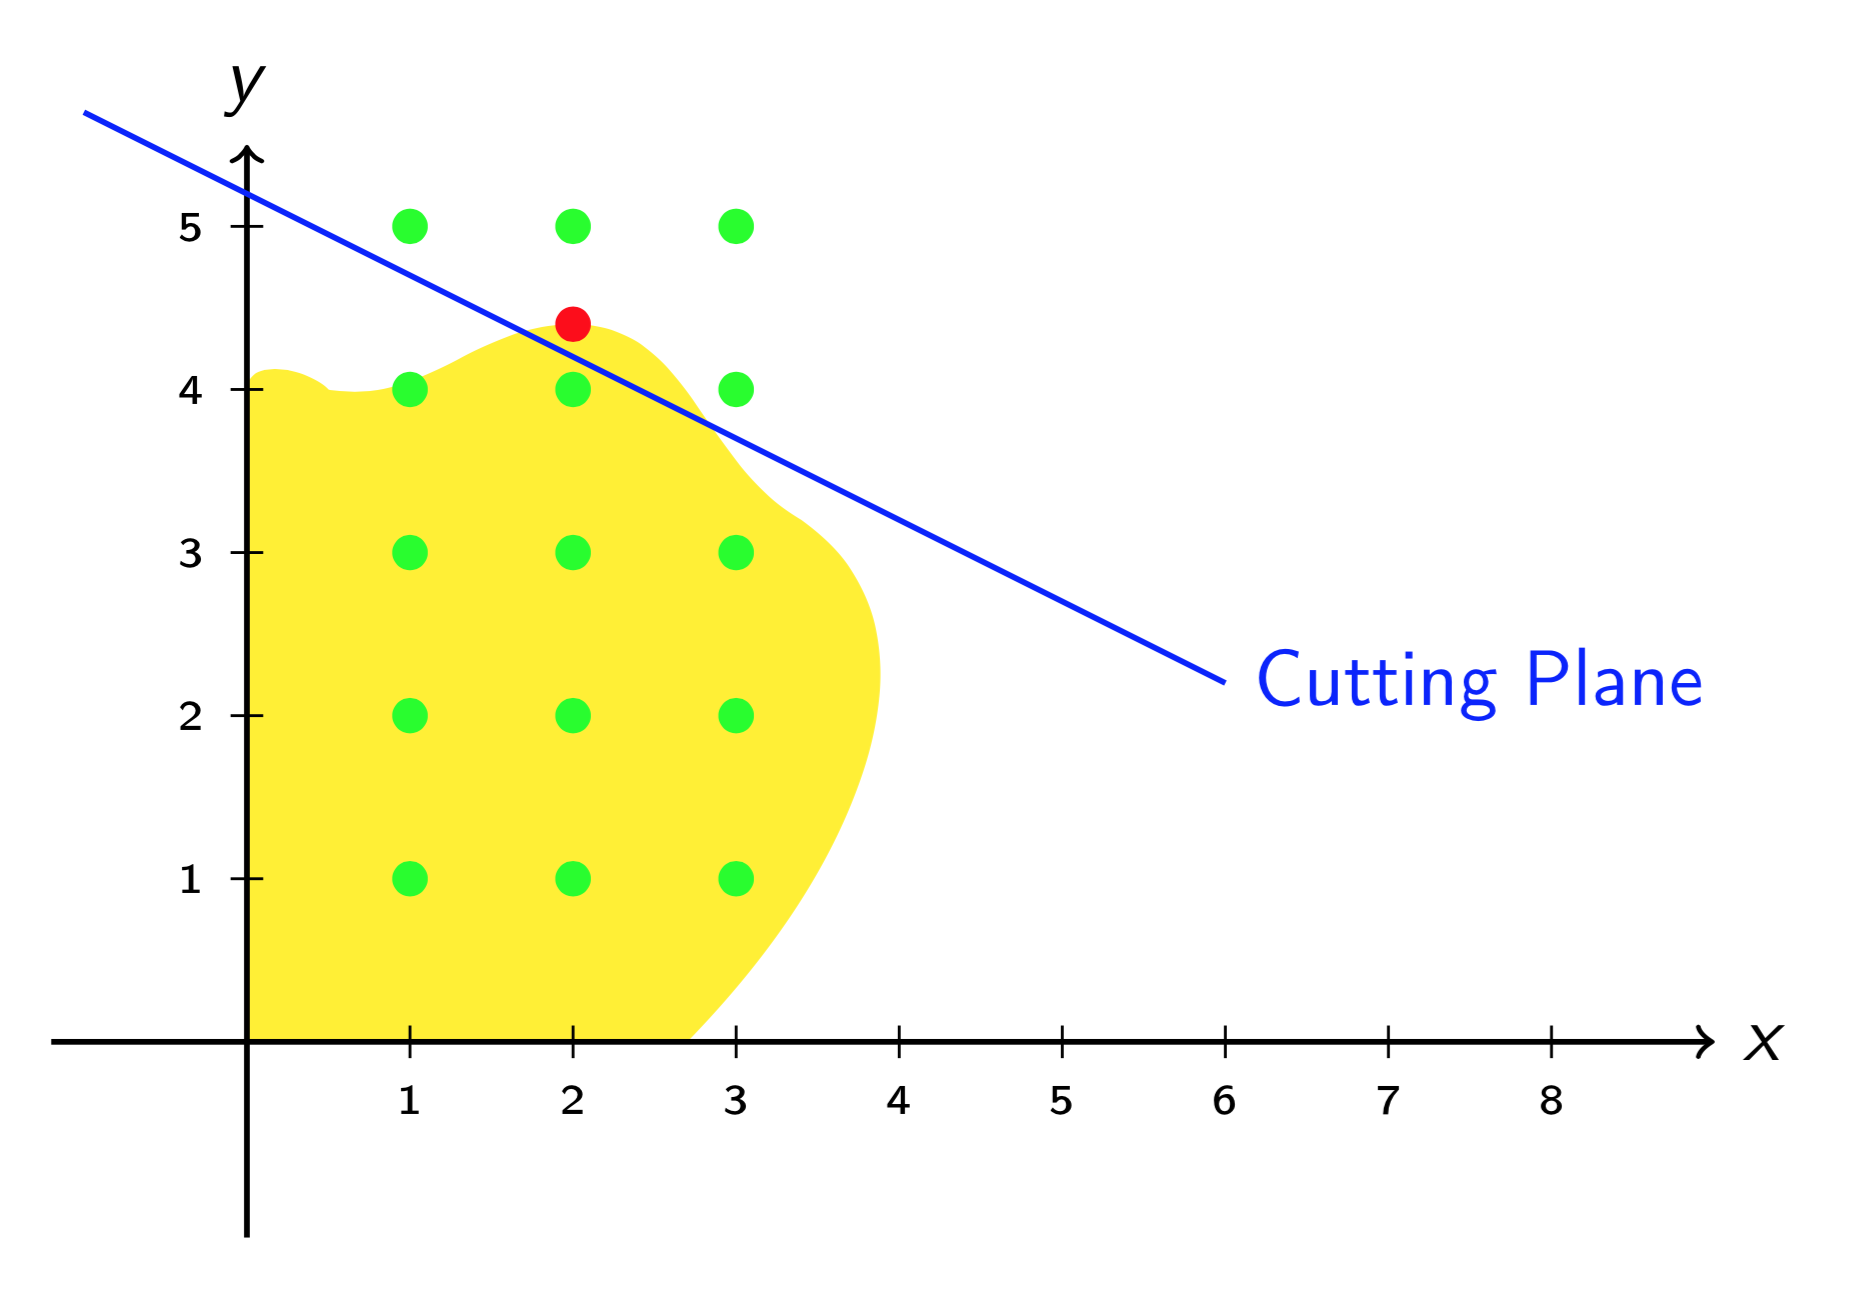
\includegraphics[width=\linewidth,height=150px,keepaspectratio]{schnittebenen_2.png}
  \caption{Einfügen einer korrekten Schnittebene}
  \label{img:cutting_planes_2}
\end{figure}

Dabei darf keine mögliche, ganzzahlige Lösung abgeschnitten werden.
Im Allgemeinen wird ein Problem durch $2^n$ Schnittebenen gelöst, jedoch werden
typischerweise nur $n$ verletzte Schnittebenen generiert, damit alle exponentiell
vielen Schnittebenen erfüllt sind. Ein Nachteil des Schnittebenenverfahrens
ist, dass selbst nach dem Einfügen der Schnittebenen keine ganzzahlige Lösung
besteht.

\subsubsection{Branch and Cut}
Um die Schwächen des Schnittebenenverfahrens und der Branch and Bound-Methode
zu adressieren (hohe Laufzeit, teilweise nicht-ganzzahlige Lösungen) wurden
beide Verfahren miteinander zum \textit{Branch and Cut} Verfahren kombiniert.
Dieses Verfahren beginnt auch bei einer relaxierten Lösung, nur wird hier
zunächst versucht mit Schnittebenen zu einer ganzzahligen Lösung zu kommen,
um nicht verzweigen zu müssen und somit erneut ein LP lösen zu müssen. Sollte
nach Anwendung der Schnittebenen keine ganzzahlige Lösung entstehen, so wird,
wie bei Branch and Bound, in zwei Substränge verzweigt, auf die das Verfahren
dann wiederum angewandt wird.
Insgesamt resultiert dies in deutlich geringeren Laufzeiten.

\section{Praktische Anwendungen mit Concorde}
Eine bekannte Umsetzung dieser Algorithmen erfolgte im Programm \textit{Concorde}.
Concorde wurde von David Applegate, Robert E. Bixby, Vašek Chvátal und William J. Cook
in C entwickelt und ist eines der besten exakten TSP-Lösungsprogramme.
Concorde verwendet grundlegend auch das Branch and Cut Verfahren.
Dabei lässt Concorde mehrere Formen der Relaxierung
zu: So werden die $2^n$ Bedingungen gegen
Kurzkreiszyklen nicht direkt komplett eingesetzt, sondern erst Schritt für Schritt.
Zudem lässt Concorde es zu, dass Kanten zwischen zwei Knoten kontinuierlich gewählt
werden können, wie zum Beispiel $0.5 \cdot$ Kante A. Um nicht alle Kanten von Beginn
an als mögliche Kanten zu behandeln,
verwendet Concorde die \textit{Delaunay-Triangulation}.
Die Delaunay-Triangulation ist ein Verfahren, um aus einer Punktemenge ein Dreiecksnetz
zu erstellen. Für die Lösung eines TSP liefert das den Vorteil, dass alle Kanten, die
in diesem Netz enthalten sind, auch in der späteren, optimalen Tour enthalten sind und
nicht alle Kanten betrachtet werden müssen.

\begin{figure}
  \centering
  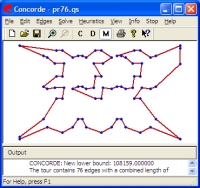
\includegraphics[width=\linewidth,height=150px,keepaspectratio]{tsp_concorde.jpg}
  \caption{Screenshot Concorde TSP-Solver}
  \label{img:cutting_planes_2}
\end{figure}


\end{document}